\graphicspath{{3analytic/asy/}}

\section{Analytic Geometry}

Geometry in the style of Euclid and Hilbert is \emph{synthetic}: axiomatic, without co-ordinates or explicit numerical measures of angle, length, area or volume. By contrast, the modern practice of geometry is typically \emph{analytic}: reliant on algebra and co-ordinates (including vectors). The critical development came in the early 1600s courtesy of René Descartes and Pierre de Fermat: the \emph{axis} as a fixed reference ruler against which objects can be measured using \emph{co-ordinates.}

\subsection{The Cartesian Co-ordinate System}

Since Cartesian geometry (\emph{Descartes'} geometry) should be familiar, we merely sketch the core ideas.

\begin{itemize}\itemsep2pt
  \begin{minipage}[t]{0.72\linewidth}\vspace{-5pt}
  	\item Perpendicular \emph{axes} meet at the \emph{origin} $O$.
  	\item The \emph{co-ordinates} of a point are measured by projecting onto the axes; since these are real numbers we denote the set of these
  	\[
  		\R^2=\bigl\{(x,y):x,y\in\R\bigr\}
  	\]
  	In the picture, $P$ has co-ordinates $(1,2)$; we usually write $P=(1,2)$.
  	\item Algebra is introduced via \emph{addition} and \emph{scalar multiplication}
	\end{minipage}
	\hfill
	\begin{minipage}[t]{0.27\linewidth}\vspace{-5pt}
		\flushright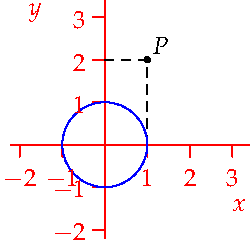
\includegraphics{analytic-axes}
	\end{minipage}\par\vspace{-15pt}
  \begin{gather*}
  	P+Q =(p_1,p_2)+(q_1,q_2) =(p_1+q_1,p_2+q_2)\qquad
  	\lambda P=(\lambda p_1,\lambda p_2)
  \end{gather*}
  \item The \emph{length} of a segment uses Pythagoras' Theorem%\footnotemark
  \[
  	d(P,Q) =\nm{PQ} =\sqrt{(q_1-p_1)^2+(q_2-p_2)^2}
  \]
  In the picture, $\nm{OP}=\sqrt{1^2+2^2}=\sqrt 5$. As in Section \ref{sec:similar}, segments are congruent if and only if they have the same length.

  \item \emph{Curves} are defined using \emph{equations.} E.g., $x^2+y^2=1$ describes a circle. 
\end{itemize}

Analytic geometry was originally conceived as a computational toolkit built on top of Euclid. Mathematicians at first felt the need to justify analytic arguments synthetically lest no-one believe their work.\footnote{%
	An attitude which persisted for some time: the presentation in Issac Newton's groundbreaking \emph{Principia} (1687) was largely synthetic, even though his private derivations made extensive use of co-ordinates and algebra.%
} Synthetic geometry is not without its benefits, but its study has increasingly become a fringe activity; co-ordinates are just too useful to ignore. We may therefore assume anything from Euclid and mix strategies as appropriate. To see this at work, consider a simple result.

\begin{minipage}[t]{0.74\linewidth}\vspace{0pt}
	\begin{lemm}{}{cart-para}
		Non-collinear points $O=(0,0)$, $A=(x,y)$, $B=(v,w)$ and $C:=(x+v,y+w)$, form a parallelogram $OACB$.
	\end{lemm}
	
	\begin{proof}
		Opposite sides have the same length ($\nm{BC}=\sqrt{x^2+y^2}=\nm{OA}$, etc.) and are thus congruent. SAS shows $\triangle OAC\cong \triangle CBO$. Euclid's discussion of alternate angles (pages \pageref{defn:parallel}--\pageref*{axiom:playfair}) forces opposite sides to be parallel.
	\end{proof}
\end{minipage}
\hfill
\begin{minipage}[t]{0.25\linewidth}\vspace{0pt}
	\flushright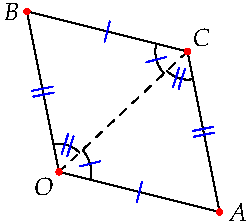
\includegraphics[scale=0.9]{analytic-para}
\end{minipage}\medbreak

Lemma \ref{lemm:cart-para} is essentially vector addition: feel free to use such notation/language if you prefer.

\goodbreak


\iffalse
\boldsubsubsection{Vector Geometry}

Vectors come to us courtesy of several mathematicians, most prominently William Rowan Hamilton (1805--1865), Oliver Heaviside (1850--1925) and J.~Willard Gibbs (1839--1903). Hamilton had stumbled upon the algebra of \emph{quaternions} when attempting to extend to three dimensions the contemporary use of complex numbers (Section \ref{sec:complexplane}) to describe plane geometry.\footnote{Quaternions are objects of the form $a+bi+cj+dk$ where $a,b,c,d\in\R$, $i^2=j^2=k^2=-1$ and $i,j,k$ multiply as if using the cross-product ($ij=k=-ji$, etc.). Hamilton couldn't make the three-dimensional part ($a=0$) into a suitable algebra, but a fourth dimension fixed things. Hamilton eventually realized that if he dropped his requirement of having a well-defined multiplication, he could apply his vector approach to the study of geometry in any dimension. %Hamilton is also famous for reformulating classical mechanics into the \emph{Hamiltonian mechanics} beloved by modern Physicists.
} Heaviside and Gibbs %(an Englishman and an American) 
independently developed vector calculus. The revolution was rapid; by 1900 vector calculations were dominant in physics. 

\begin{defn}{}{}
A \emph{directed line segment} $\rayv{AB}$ is a segment together with an \emph{orientation.}\footnotemark\smallbreak
The \emph{position vector} of a point $A$ is the directed line segment $\rayv{OA}$ where $O$ is the origin.\smallbreak
A \emph{vector} is an equivalence class of directed line segments where two segments are equivalent if and only if they are congruent and oriented in the same direction.
\end{defn}

\footnotetext{We write $\rayv{AB}$ for the directed line segment so as to distinguish it from the \emph{ray} $\ray{AB}$ of Hilbert's Euclidean geometry.}

A vector has \emph{length} and \emph{direction}, but no fixed location. All directed line segments with the same length and direction represent the same vector. The \emph{standard representation} of a vector involves placing its \emph{tail} at the origin; we may then describe the vector by giving the co-ordinates of its \emph{head.}

\begin{example}[lower separated=false, sidebyside, sidebyside align=top seam, sidebyside gap=0pt, righthand width=0.3\linewidth]{}{}
In the picture, the standard representation of a vector $\vv$ is shown in blue. The green arrows are other representations of the same vector. Various common notations include
\[\vv=\vec{\mathrm{v}}=\underline{\mathrm{v}}=\rayv{OA}=\twovec 21=\ip{2,1}=2\vi+\vj\]
The usual convenient abuse of terminology is at work: strictly $\rayv{OA}\in\vv$ since $\vv$ is an equivalence class, but no-one writes this.
\tcblower
\flushright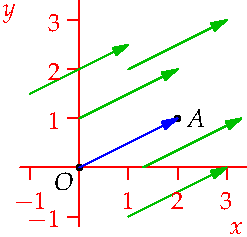
\includegraphics{analytic-defn}
\end{example}

Addition and scalar multiplication are defined algebraically in the familiar manner:\par
\begin{minipage}[t]{0.74\linewidth}\vspace{-5pt}
\[\vv+\vw=\twovec{v_1}{v_2}+\twovec{w_1}{w_2}=\twovec{v_1+w_1}{v_2+w_2},\qquad \lambda\vv:=\twovec{\lambda v_1}{\lambda v_2}\]
Vector addition can be visualized by placing representative segments \emph{nose-to-tail}. In view of Lemma \ref{lemm:cart-para}, the commutativity of addition $\vv+\vw=\vw+\vv$ is often known as the \emph{parallelogram law.} Indeed the Lemma may be rephrased in this language: the parallelogram $OACB$ is \emph{spanned by}
\[\rayv{OA}=\twovec xy\quad\text{and}\quad\rayv{OB}=\twovec vw\]
\end{minipage}
\begin{minipage}[t]{0.25\linewidth}\vspace{0pt}
\flushright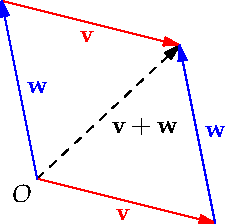
\includegraphics{analytic-para2}
\end{minipage}\medbreak
The scalar multiple $\lambda\vv$ may be viewed as stretching or shrinking $\vv$, and reversing its direction when $\lambda<0$.

\goodbreak

\fi


\begin{lemm}{}{lineparam}
	The points $X_t$ on the line $\lin{PQ}$ are in 1--1 correspondence with the real numbers via 
	\[
		X_t= P+t(Q-P)=(1-t)P+tQ
	\]
	Moreover, $d(P,X_t)=\nm t\nm{PQ}$ so that $t$ measures the (signed) distance along the line.
\end{lemm}

The proof is an exercise. As an example of how easy it can be to work in analytic geometry, we apply the Lemma to re-establish a famous result (compare Exercise \ref*{sec:similar}.\ref{exs:centroideuclid2} where we used Ceva's Theorem!).

\begin{thm}{}{centroidanalytic}
	The medians of a triangle meet at a point $2/3$ of the way along each median.
\end{thm}


\begin{proof}
	Given $\triangle ABC$, label the midpoints of each side as shown. By Lemma \ref{lemm:lineparam}, these are\par
	\begin{minipage}[t]{0.7\linewidth}\vspace{-8pt}
		\[
			M=\frac 12(B+C),\quad N=\frac 12(A+B),\quad P=\frac 12(A+C)
		\]
		The point $\frac 23$ of the way along median $\cl{AM}$ is then
		\[
			G:=A+\frac 23(M-A)=A+\frac 23(B+C-2A)=\frac 13(A+B+C)
		\]
	\end{minipage}
	\hfill
	\begin{minipage}[t]{0.29\linewidth}\vspace{-23pt}
		\flushright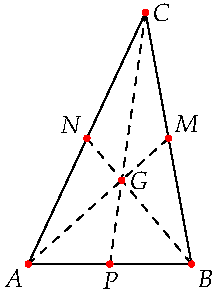
\includegraphics[scale=0.95]{analytic-centroid}
	\end{minipage}\medbreak
		By symmetry (check directly if you like!), $G$ is also $\frac 23$ of the way along the other two medians.
\end{proof}

Our proof relied on adding points as abstract objects, though we could instead have expressed $A,B,C,\ldots$ in co-ordinates. Exercise \ref{exs:centroidcoord} does exactly this in an approach that illustrates one of the biggest advantages of analytic geometry: the freedom to choose axes and co-ordinates so as to make calculations simple. This is essentially Euclid's superposition principle or Hilbert's \emph{congruence} in disguise: we'll make this correspondence rigorous in Section \ref{sec:klein} when we discuss \emph{isometries}.

\begin{exercises}
	\exstart By completing the square, identify the curve described by the equation
	\[
		x^2+y^2-4x+2y=10
	\]
	
	\begin{enumerate}\setcounter{enumi}{1}
	  \item\label{exs:centroidcoord}\begin{enumerate}
	  	\item Perform a pure co-ordinate proof of Theorem \ref{thm:centroidanalytic}. For simplicity, arrange the triangle so that $A=(0,0)$ is the origin, and $B$ points along the positive $x$-axis.
	  
			\item Descartes and Fermat did not have a fixed perpendicular second axis! Their approach was equivalent to choosing a second axis oriented to make the problem as simple as possible.\par
			Given $\triangle ABC$, choose axes pointing along $\cl{AB}$ and $\cl{AC}$. Describe the co-ordinates of $B$ and $C$ with respect to such axes. Now give an even simpler proof of the centroid theorem (\ref{thm:centroidanalytic}).
	  \end{enumerate}

	
		\item Prove Lemma \ref{lemm:lineparam}.

	
		\item A \emph{parabola} is a curve whose points are equidistant from a fixed point $F$ (the \emph{focus}) and a fixed line $\ell$ (the \emph{directrix}).
		\begin{enumerate}
		  \begin{minipage}[t]{0.73\linewidth}\vspace{-2pt}
			   \item Choose axes as shown in the picture so that $F=(0,a)$ and $\ell$ has equation $y=-a$. Find the equation of the parabola.
			   \item Now let $e$ be a positive constant ($\neq 0,1$). What happens if $\ell$ has equation $y=-\frac ae$ and $\frac{\nm{PF}}{\nm{F\ell}}=e$? What happens in the limit $e\to 0^+$?
			\end{minipage}
			\hfill
			\begin{minipage}[t]{0.25\linewidth}\vspace{-10pt}
				\flushright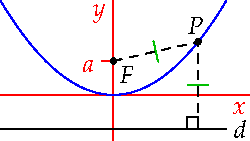
\includegraphics[scale=0.95]{analytic-parabola}
			\end{minipage}
		\end{enumerate} 
	
	\end{enumerate}
\end{exercises}


\clearpage


\subsection{Angles and Trigonometry}\label{sec:analyticangle}

Angles are defined differently to Section \ref{sec:similar}, though the approach should feel familiar. %We use radians, angles are \emph{oriented} and may be \emph{reflex} (larger than a straight edge). 

\begin{defn}[lower separated=false, sidebyside, sidebyside align=top seam, sidebyside gap=0pt, righthand width=0.32\linewidth]{}{}
	Suppose $A,B,C$ are distinct points in the plane. Take any \textcolor{blue}{circular arc} centered at $A$ and define the \emph{radian measure}
	\[
		\measuredangle BAC:=\frac{\text{\textcolor{blue}{arc-length}}}{\text{radius}} \in[0,2\pi)
	\]
	where arc-length is measured \emph{counter-clockwise} from $\ray{AB}$ to $\ray{AC}$.
	\tcblower
	\flushright
	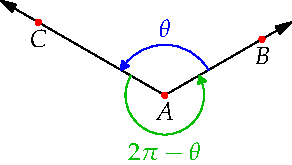
\includegraphics{angles-example}
\end{defn}

Since arc-length scales with radius, the definition is independent of the radius of the circular arc. It is important to appreciate the difference between angle measures in our two geometries.\vspace{-5pt}

\begin{description}\itemsep0pt
  \item[Euclidean geometry] All angles $<\ang{180}$. Reversed legs $\rightsquigarrow$ \emph{congruent} angles and \emph{same degree measure}:
  \[
  	\angle CAB\cong\angle BAC\iff m\angle CAB=m\angle BAC
  \]
  \item[Analytic geometry] Reflex angles exist ($\ge\pi$). Reversed legs $\rightsquigarrow$ \emph{different radian measure}:
  \[
  	\measuredangle CAB=2\pi-\theta=2\pi-\measuredangle BAC \neq \measuredangle BAC \tag{unless a straight edge}
  \]
	\begin{minipage}[t]{0.79\linewidth}\vspace{-5pt}
  	In the picture, $\textcolor{Green}{\measuredangle CAB}$ is \textcolor{red}{not} the radian measure ($	\textcolor{blue}{\theta}$) of $\angle CAB$! However,
  	\[
			\tcbhighmath{\text{Angles congruent $\Longleftrightarrow$ radian measures equal and $<\pi$}}
		\]
		As such, it is common to label angles in a triangle by their radian measure; standard convention is shown: e.g., ($A$, $a$, $\alpha$) for (point, length, angle).%\smallbreak
	%Trigonometric functions may now be defined for all angles simultaneously.
	\end{minipage}
	\hfill
	\begin{minipage}[t]{0.2\linewidth}\vspace{-17pt}
		\flushright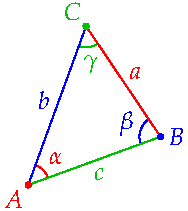
\includegraphics{angle-notation}
	\end{minipage}
\end{description}




\begin{defn}[lower separated=false, sidebyside, sidebyside align=top seam, sidebyside gap=0pt, righthand width=0.23\linewidth]{Trigonometric Functions}{}
	Let $O$ be the origin and $I=(1,0)$. Let $P=(x,y)$ lie on a circle of radius $r$ and $\theta=\measuredangle IOP$. We define:
	\[
		\cos\theta :=\frac xr\qquad \sin\theta:=\frac yr\qquad \tan\theta:=\frac yx\quad (x\neq 0)
	\]
	AAA similarity (Thm.\,\ref{thm:aaasim}) says these are well-defined, independent of $r$.
	\tcblower
	\flushright
	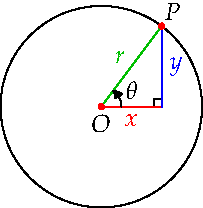
\includegraphics[scale=0.95]{angles-sine}
\end{defn}

\begin{example}{}{}
	Basic trig identities should be obvious from the picture: e.g.,
	\[
		\cos^2\theta+\sin^2\theta=1 \text{ (Pythagoras!)}
		\quad\text{and}\quad
		\sin\theta=\cos(\tfrac\pi 2-\theta)
	\]
	Which well-known facts regarding sine and cosine are illustrated by the following?
	\begin{center}
		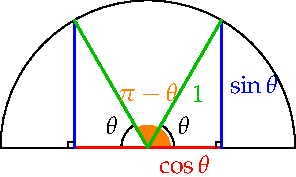
\includegraphics[scale=0.95]{angles-trigbasic1}
		\qquad
		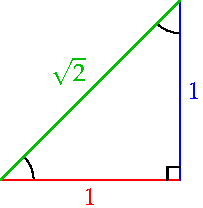
\includegraphics[scale=0.95]{angles-trigbasic2}
		\qquad
		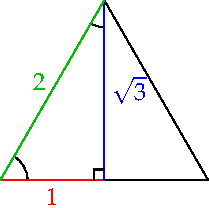
\includegraphics[scale=0.95]{angles-trigbasic3}
	\end{center}
\end{example}

\goodbreak


\boldinline{Solving Triangles}

A triangle is described by six values: three side lengths and three angle measures. Euclid's triangle congruence theorems (SAS, ASA, SSS, SAA) say that three of these in suitable combination are enough to recover the rest. In analytic geometry, these calculations typically use the sine and cosine rules.

\begin{thm}{}{cosinerule}
	Label the sides/angles of $\triangle ABC$ following the standard convention (page \pageref{sec:analyticangle}):
	\begin{description}
		\item[\normalfont\emph{Sine Rule}] If $d$ is the diameter of the circumcircle (Defn.\ \ref{defn:circledef}), then \ \smash{$\displaystyle\frac{\sin\alpha}a=\frac{\sin\beta}b=\frac{\sin\gamma}c=\frac 1d$}
		\item[\normalfont\emph{Cosine Rule}] $c^2=a^2+b^2-2ab\cos\gamma$
	\end{description}
\end{thm}


\begin{minipage}[t]{0.72\linewidth}\vspace{0pt}
	\begin{proof}
		We prove the sine rule and leave the cosine rule as an exercise. Everything relies on Corollary \ref{cor:thalescor}. Draw the circumcircle of $\triangle ABC$. Construct $\triangle BCD$ with diameter $\cl{BD}$; this is right-angled at $C$ by Thales' Theorem. There are two cases:
		\begin{enumerate}
		  \item If $A$ and $D$ lie on the same side of $\lin{BC}$, then they share the same arc. But then $\measuredangle BDC=\alpha$ and
		  \[
		  	a=d\sin\measuredangle BDC=d\sin\alpha
		  \]
		  \item If $A$ and $D$ lie on opposite sides of $\lin{BC}$, then the quadrilateral $ABDC$ lies on a circle. Opposite angles at $A,D$ are supplementary, whence
			\[
				\sin\alpha=\sin(\pi-\alpha)=\sin\measuredangle BDC=\frac ad
			\]
		\end{enumerate}
		The two other angle-side combinations follow by permutation.\phantom{\qedhere}
	\end{proof}
\end{minipage}
\hfill
\begin{minipage}[t]{0.25\linewidth}\vspace{-5pt}
	\flushright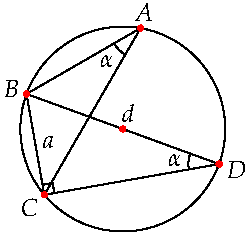
\includegraphics[scale=0.95]{angles-sinerule}\smallbreak
	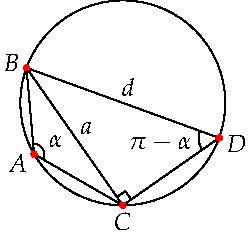
\includegraphics[scale=0.95]{angles-sinerule2}\\[-20pt]
	\hfill\qedsymbol
\end{minipage}


\begin{examples}{}{trisolve}
	\exstart Given SSS data, we may compute the three angles using the cosine rule. For instance the given triangle has
	\begin{enumerate}\setcounter{enumi}{1}
		\begin{minipage}[t]{0.86\linewidth}\vspace{-13pt}
		  \item[]
		  \begin{gather*}
				\alpha=\frac{6^2+7^2-3^2}{2\cdot 6\cdot 7}=\cos^{-1}\frac{19}{21}\approx\ang{25}\qquad
				\beta=\frac{3^2+7^2-6^2}{2\cdot 3\cdot 7}=\cos^{-1}\frac{11}{21}\approx\ang{58}\\[5pt]
				\gamma=\frac{3^2+6^2-7^2}{2\cdot 3\cdot 6}=\cos^{-1}\frac{-1}{9}\approx\ang{96}
			\end{gather*}
			Once you have $\alpha$, you could alternatively switch to the sine rule to find $\beta$, before computing $\gamma=\pi-\alpha-\beta$.
		\end{minipage}\hfill\begin{minipage}[t]{0.13\linewidth}\vspace{-24pt}
			\flushright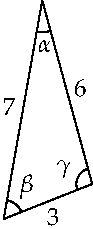
\includegraphics[scale=0.95]{angles-ssssolve}
		\end{minipage}\smallbreak
		\begin{minipage}[t]{0.75\linewidth}\vspace{0pt}
			\item\label{ex:trisolve2} To solve the given triangle with ASA data, first find the remaining angle $\textcolor{Green}{\gamma}=\pi-\textcolor{red}{\frac\pi 4}-\textcolor{blue}{\frac\pi 3} =\textcolor{Green}{\frac{5\pi}{12}}$ before applying the sine rule
		  \begin{align*}
		  	\textcolor{red}{\frac{\sin\frac\pi 4}a} 
		  		=\textcolor{blue}{\frac{\sin\frac\pi 3}b} 
		  		=\textcolor{Green}{\sin\frac{5\pi}{12}}%=\textcolor{Green}{\cos\frac{\pi}{12}}
		  		\implies 
		  	&\textcolor{red}{a}
		  		=\frac 1{\sqrt 2\sin\frac{5\pi}{12}}\approx 0.732\\
		  	&\textcolor{blue}{b}
		  		=\frac{\sqrt 3}{2\sin\frac{5\pi}{12}}\approx 0.897
		  \end{align*}
		\end{minipage}\hfill\begin{minipage}[t]{0.24\linewidth}\vspace{0pt}
			\flushright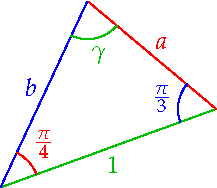
\includegraphics[scale=0.95]{angles-asasolve}
		\end{minipage}
	\end{enumerate}
\end{examples}


\goodbreak



\begin{minipage}[t]{0.63\linewidth}\vspace{-10pt}
	\boldinline{Multiple-angle formulæ}\phantomsection\label{sec:multangle}
	
	The picture provides a very simple proof of the expressions
	\begin{gather*}
		\sin(\alpha+\beta)=\textcolor{Green}{\sin\alpha\cos\beta}+\textcolor{blue}{\cos\alpha\sin\beta}\\
		\cos(\alpha+\beta)=\cos\alpha\cos\beta-\sin\alpha\sin\beta
	\end{gather*}
	at least when $\alpha+\beta<\frac\pi 2$. A little algebraic manipulation produces the double-angle and difference formulæ, and verifies that these hold for all possible angle inputs.
\end{minipage}
\hfill
\begin{minipage}[t]{0.36\linewidth}\vspace{0pt}
	\flushright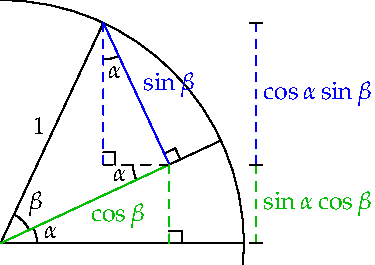
\includegraphics[scale=0.85]{angles-multipleangle}
\end{minipage}\par
\begin{align*}
	&\sin 2\alpha=2\sin\alpha\cos\alpha &&\sin(\alpha-\beta)=\sin\alpha\cos\beta-\cos\alpha\sin\beta\\
	&\cos 2\alpha=\cos^2\alpha-\sin^2\alpha=2\cos^2\alpha-1&&\cos(\alpha-\beta)=\cos\alpha\cos\beta+\sin\alpha\sin\beta
\end{align*}

\smallskip

\begin{exercises}{}{}
	\exstart A triangle has angle of $\frac{2\pi}3$ radians between sides of lengths 2 and $\sqrt 3-1$. Find the length of the remaining side, and the remaining angles.\vspace{-2pt}
	\begin{enumerate}\setcounter{enumi}{1}	
		\item Describe how to solve a triangle given data in line with the SAA congruence theorem.
		
		
		\item Two measurements for the height of a mountain are taken at sea level 5000\,ft apart in a line pointing away from the mountain. The angles of elevation to the mountain top from the horizontal are \ang{15} and \ang{13} respectively. What is the height of the mountain?
		
		
		\item Use a multiple angle formula to find an exact value for $\cos\frac{\pi}{12}$ and thus exact values for the side lengths of the triangle in Example \ref*{ex:trisolve}.\ref{ex:trisolve2}.
		
		
		\item The area of a triangle is $\frac 12$(base)$\cdot$(height). By using each side of the triangle alternately as the `base,' find an alternative proof of the sine rule without the relationship to the circumcircle. 
		
		
		\item You are given SSA data for a triangle: sides with lengths $a=1$ and $b=\sqrt 3$ and angle $\alpha=\frac\pi 6$. Show that there are \emph{two} triangles satisfying this data. Can you generalize to general SSA data?
		 
	
		\begin{minipage}[t]{0.72\linewidth}\vspace{-8pt}	
			\item\begin{enumerate}
			  \item By dropping a perpendicular from $B$ to $\lin{AC}$ at $D$ and applying the Pythagorean theorem, construct a proof of the cosine rule.
		 		
		 		\item Is your argument valid if $D$ is not interior to $\cl{AC}$? Explain.
			\end{enumerate}
		\end{minipage}
		\hfill
		\begin{minipage}[t]{0.27\linewidth}\vspace{-12pt}
			\flushright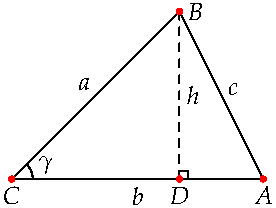
\includegraphics[scale=0.8]{angles-cosrule}
		\end{minipage}
	
		\item The \emph{dot product} of $A=(a_1,a_2)$ and $B=(b_1,b_2)$ is $A\cdot B:=a_1b_1+a_2b_2$. Apply the cosine rule to $\triangle OAB$ to prove that
		\[
			A\cdot B=\nm{OA}\nm{OB}\cos\measuredangle AOB
		\]
		
		
		\item Derive the multiple-angle formula for $\sin(\alpha-\beta)$.\par
		(\emph{Remember that $0\le \alpha,\beta, \alpha-\beta<2\pi$ so you can't simply switch the sign of $\beta$!})
		
		
		\begin{minipage}[t]{0.7\linewidth}\vspace{0pt}
			\item Given the arrangement pictured, find $x$, the radian-measure $\alpha$ and the exact value of $\cos\alpha$.\par
			(\emph{Hint: first show that you have similar isosceles triangles})	
		\end{minipage}
		\hfill
		\begin{minipage}[t]{0.29\linewidth}\vspace{0pt}
			\flushright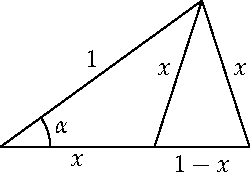
\includegraphics[scale=0.9]{angles-sin36}
		\end{minipage}
	\end{enumerate}
\end{exercises}

\clearpage



\subsection{Isometries}\label{sec:klein}

At the heart of elementary geometry is \emph{congruence}, the idea that geometric figures can be essentially the same without necessarily being equal. In analytic geometry, congruence may be described algebraically using \emph{functions}. This follows from the fact that two segments have the same length if and only if they are congruent.

\begin{defn}{}{}
	A function $f:\R^2\to\R^2$ is a \emph{(Euclidean) isometry} if it preserves lengths:\footnotemark
	\[
		\forall P,Q\in\R^2,\ d\bigl(f(P),f(Q)\bigr)=\nm{PQ}
	\]
	Two figures (segments, angles, triangles, etc.) are \emph{congruent} precisely when there is an isometry $f:\R^2\to\R^2$ mapping one to the other.
\end{defn}

\footnotetext{%
	In ancient Greek, \emph{iso-metros} is literally \emph{same measure (length/distance)}.}


\begin{example}{}{isomsetup}
	We check that the map $f(x,y)=\frac 15\bigl(3x+4y,4x-3y\bigr)+(3,1)$ is an isometry. If $P=(x,y)$ and $Q=(v,w)$, then
	\begin{align*}
		d\bigl(f(P),f(Q)\bigr)^2&=\smash[t]{\left(\frac{3v+4w-3x-4y}5\right)^2+\left(\frac{4v-3w-4x+3y}5\right)^2}\\
		&=\frac{3^2+4^2}{5^2}\bigl((v-x)^2+(w-y)^2\bigr) =\nm{PQ}^2
	\end{align*}
\end{example}

Isometric segments are certainly congruent. We should make sure the same holds for angles.

\begin{lemm}{}{isomlinepreserve}
	Isometries preserve (non-oriented) angles: if $f:\R^2\to\R^2$ is an isometry, then
	\[
	  \angle PQR\cong \angle f(P)f(Q)f(R)
	\]
\end{lemm}

\begin{proof}
Since $f$ is an isometry, the sides of $\triangle PQR$ and $\triangle f(P)f(Q)f(R)$ are mutually congruent in pairs. The SSS triangle congruence theorem says that the angles are also mutually congruent.%\smallbreak
% For part 2, let $t\in\R$ and consider the point $X_t=(1-t)P+tQ$.
% \begin{itemize}
%   \item Since $\nm{PX_t}=\nm{-t(P-Q)}=\nm{t}\nm{PQ}$, the point $f(X_t)$ must lie on the \emph{circle} with radius $\nm{t}\nm{PQ}$ centered at $f(P)$.
%   \item Similarly $\nm{X_tQ}=\nm{1-t}\nm{PQ}\implies f(X_t)$ lies on the circle centered at $f(Q)$ with radius $\nm{1-t}\nm{PQ}$.
% \end{itemize}
%  Since $f$ preserves distances, these circles have a unique intersection point: that is,
%  \[f(X_t)=(1-t)f(P)+tf(Q)\tag*{\qedhere}\]
\end{proof}



\begin{example*}[lower separated=false, sidebyside, sidebyside align=top seam, sidebyside gap=0pt, righthand width=0.32\linewidth]{\ref{ex:isomsetup}, cont}{}
	\textcolor{red}{Warning}: Isometries can \emph{reverse orientation}! In the picture,
	\[
		\measuredangle ABC=\textcolor{Green}{\frac\pi 2}
		\quad\text{but}\quad
		\measuredangle f(A)f(B)f(C)=\textcolor{Green}{\frac{3\pi}2}=2\pi-\measuredangle ABC
	\]
	\tcblower
	\flushright
	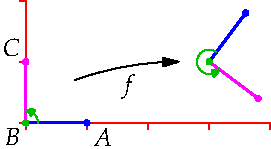
\includegraphics{isom-refl2}
\end{example*}

Our next task is to confirm our intuition that isometries are rotations, reflections and translations. Given an isometry $f$, define $g(X)=f(X)-f(O)$, where $O$ is the origin. Then $g$ is an isometry
\[
	g(P)-g(Q)=f(P)-f(Q)\implies d\bigl(g(P),g(Q)\bigr)=d\bigl(f(P),f(Q)\bigr)=\nm{PQ}
\]
which moreover \emph{fixes the origin}: $g(O)=O$. We conclude that every isometry $f$ is the composition of an \emph{origin-preserving} isometry $g$ followed by a \emph{translation} ``$+C$:''
\[
	f(X)=g(X)+C
\]

\goodbreak

It thus suffices to describe the origin-preserving isometries $g$. For these, we make two observations.
\begin{enumerate}
	\begin{minipage}[t]{0.68\linewidth}\vspace{0pt}
	  \item\label{affinity} Suppose $\nm{OQ}=1$ and let $X_r=rQ$ for some $r\in\R$. Then
	  \begin{itemize}
	    \item $g(X_r)$ is a distance $\textcolor{blue}{\nm r=\nm{OX_r}}$ from the origin $O=g(O)$.
	    \item $g(X_r)$ is a distance $\textcolor{Green}{\nm{1-r}=\nm{QX_r}}$ from $g(Q)$.
	  \end{itemize}
	  $g(X_r)$ therefore lies on the intersection of two circles, which intersect at a single point: we conclude that
	  \[
	  	g(rQ)=rg(Q)
	  \]
	  The picture shows the case $0<r<1$, where the uniqueness of intersection follows from
	  $1=\nm r+\nm{1-r}$.
	\end{minipage}
	\hfill
	\begin{minipage}[t]{0.31\linewidth}\vspace{0pt}
		\flushright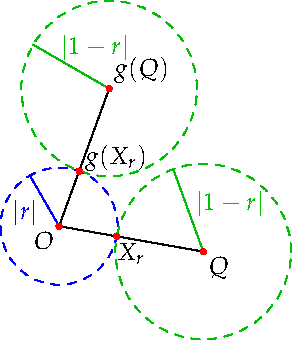
\includegraphics[scale=0.95]{isom-scale}
	\end{minipage}
	\bigbreak
	\begin{minipage}[t]{0.64\linewidth}\vspace{0pt}
		\item $g(1,0)$ lies on the unit circle and therefore has the form
		\[
			g(1,0)=S_\theta:=\bigl(\cos\theta,\sin\theta\bigr)
		\]
		for some $\theta\in[0,2\pi)$. By preservation of length and angle (Lemma \ref{lemm:isomlinepreserve}), any other point $S_\phi=(\cos\phi,\sin\phi)$ on the unit circle must therefore be mapped to one of two points
		\[
			g(\textcolor{blue}{S_\phi})=\textcolor{Green}{S_{\theta\pm\phi}} =\bigl(\cos(\theta\pm\phi),\sin(\theta\pm\phi)\bigr)
		\]
		The angle $\phi$ is transferred to one side of the ray $\ray{OS_\theta}$.
	\end{minipage}
	\hfill
	\begin{minipage}[t]{0.34\linewidth}\vspace{0pt}
		\flushright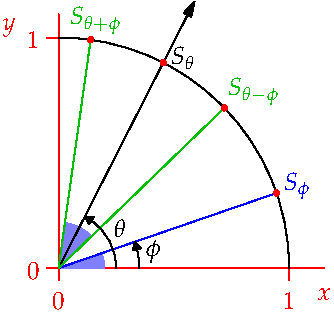
\includegraphics[scale=0.95]{isom-rot2}
	\end{minipage}
\end{enumerate}

Putting these together by writing $X=rS_\phi=(r\cos\phi,r\sin\phi)$ in polar co-ordinates, we conclude that $g$ has one of two forms:
\begin{center}
	\begin{tabular}{c@{\qquad}c}
		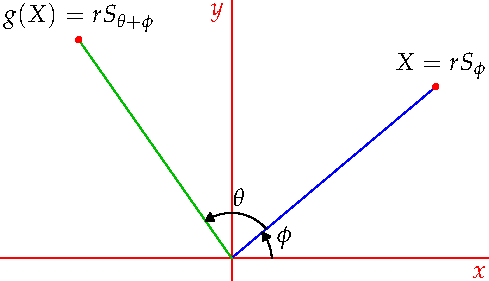
\includegraphics[scale=0.95]{isom-rot}
		&
		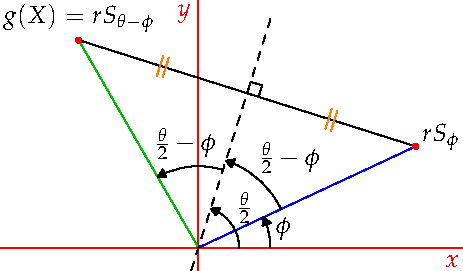
\includegraphics[scale=0.95]{isom-refl}\\
		Rotation counter-clockwise by $\theta$
		&
		Reflection across the \textcolor{Magenta}{line} making
		\\
		&
		angle $\frac\theta 2$ with positive $x$-axis
	\end{tabular}
\end{center}

\begin{thm}{}{}
	Every isometry of $\R^2$ has the form
	\[
		f(X)=g(X)+C
	\]
	where $g$ is either a rotation about the origin, or a reflection across a line through the origin. 
\end{thm}

\goodbreak


\boldsubsubsection{Calculating with isometries}

This benefits from column-vector notation and matrix multiplication. Writing $\vx=\smash{\stwovec xy =\stwovec{r\cos\phi}{r\sin\phi}}$ for the position vector of $X_r=(x,y)=rS_\phi$ and applying the multiple-angle formulæ, rotation becomes
\begin{align*}
	g(\vx)&= r\twovec{\cos(\theta+\phi)}{\sin(\theta+\phi)} =r\twovec{\cos\theta\cos\phi-\sin\theta\sin\phi}{\sin\theta\cos\phi+\cos\theta\sin\phi} =
	\begin{pmatrix}
		\cos\theta&-\sin\theta\\
		\sin\theta&\cos\theta
	\end{pmatrix}\vx
\end{align*}
For reflections, the sign of the second column is reversed:
$\begin{smatrix}
	\cos\theta&\sin\theta\\
	\sin\theta&-\cos\theta
\end{smatrix}$.
Every isometry therefore has the form $f(\vx)=A\vx+\vc$ where $A$ is an \emph{orthogonal matrix.\footnote{An orthogonal matrix satisfies $A^TA=I$. All such have the form 
$\begin{smatrix}
	\cos\theta&\mp\sin\theta\\
	\sin\theta&\pm\cos\theta
\end{smatrix}
=
\begin{smatrix}
	a&\mp b\\
	b&\pm a
\end{smatrix}$
where $a^2+b^2=1$.}}

\begin{examples}{}{isomexs}
	\exstart We revisit Example \ref{ex:isomsetup} in matrix format:
	\[
		f(\vx)=\frac 15\twovec{3x+4y}{4x-3y}+\twovec 31 =\frac 15
		\begin{pmatrix}
			3&4\\
			4&-3
		\end{pmatrix}
		\twovec xy+\twovec 31
	\]
	Since $\frac{\sin\theta}{\cos\theta}=\frac{4/5}{3/5}=\frac 43$, we see that its effect is to \emph{reflect} across the line through the origin making angle $\frac 12\tan^{-1}\frac 43\approx \ang{26.6}$ with the positive $x$-axis, before \emph{translating} by $(3,1)$.
	
	\begin{enumerate}\setcounter{enumi}{1}
		\item\label{ex:isomexs2} $\triangle_a$ has vertices $(0,0),(1,0),(2,-1)$ and is congruent to $\triangle_b$, two of whose vertices are $(1,2)$ and $(1,3)$. Find all isometries transforming $\triangle_a$ to $\triangle_b$ and the location(s) of the third vertex of $\triangle_b$.\smallbreak
	Let $f=A\vx+\vc$ be the isometry. Since $d\bigl((1,2),(1,3)\bigr)=1$ these points must be the images under $f$ of $(0,0)$ and $(1,0)$. There are \emph{four} distinct isometries:
	\smallbreak
	Cases 1,\,2:\lstsp If $f(0,0)=(1,2)$ and $f(1,0)=(1,3)$, then $\vc=f\stwovec 00=\stwovec 12$ and\par
	\begin{minipage}[t]{0.76\linewidth}\vspace{-10pt}
	  \begin{gather*}
	  	%\vc=f\twovec 00=\twovec 12,\quad 
	  	A\twovec 10+\vc=\twovec 13\implies A\twovec 10=\twovec 01   \implies A=
	  	\begin{pmatrix}
	 		0&a_{12}\\
	  	1&a_{22}
	  	\end{pmatrix}
	  \end{gather*}
	  for some $a_{12},a_{22}$. Since $A$ is orthogonal, the options are $A=
	  \begin{smatrix}
	  	0&\mp 1\\
	  	1&0
	  \end{smatrix}$
	  and we obtain two possible isometries:
	  \begin{itemize}
	    \item $\textcolor{blue}{f_1(\vx)=
	    \begin{smatrix}
	  		0&-1\\
	  		1&0
	    \end{smatrix}
	    \vx+\stwovec 12}$ rotates by \ang{90}, then translates by $\stwovec 12$.
	  	\item $\textcolor{Green}{f_2(\vx)=
	  	\begin{smatrix}
	  		0&1\\
	  		1&0
	  	\end{smatrix}
	  	\vx+\stwovec 12}$ reflects across $y=x$, then translates by $\stwovec 12$.
	  \end{itemize}
	  The third point of $\triangle_b$ is \textcolor{blue}{$f_1(2,-1)=(2,4)$} or \textcolor{Green}{$f_2(2,-1)=(0,4)$}.\medbreak
	  Cases 3,\,4: $f(0,0)=(1,3)$ and $f(1,0)=(1,2)$ results in two further isometries $\textcolor{orange}{f_3}$ and $\textcolor{Purple}{f_4}$. The details are an exercise.\medbreak
	  All four possible triangles $\triangle_b$ are drawn in the picture.
	  \end{minipage}
	  \hfill
	  \begin{minipage}[t]{0.23\linewidth}\vspace{-10pt}
	  	\flushright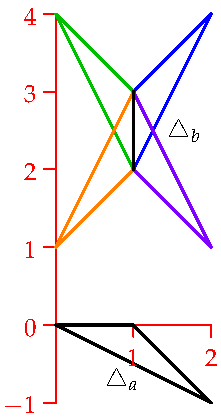
\includegraphics[scale=0.95]{isom-ex}
	  \end{minipage}
	\end{enumerate}
\end{examples}



In 1872, Felix Klein suggested that the geometry of a set is the study of its \emph{invariants}: properties preserved by its \emph{group} of structure-preserving transformations. In Euclidean geometry, this is the group of \emph{Euclidean isometries} (Exercise \ref{exs:kleingroup}). Klein's approach provided a method for analyzing and comparing the non-Euclidean geometries beginning to appear in the late 1800s. By the mid 1900s, the resulting theory of \emph{Lie groups} had largely classified classical geometries. Klein's algebraic approach remains dominant in modern mathematics and physics research.


\goodbreak



\begin{exercises}
	\exstart Let $f:\R^2\to\R^2$ be the isometry, ``reflect across the line through the origin making angle $\frac\pi 3$ with the positive $x$-axis.'' Find a $2\times 2$ matrix $A$ such that $f(\vx)=A\vx$.
	
	\begin{enumerate}\setcounter{enumi}{1}  
	  \item Describe the geometric effect of the isometry $f(\vx)=\frac 12
	  \begin{smatrix}
	  	1&\sqrt 3\\
	  	-\sqrt 3&1
	  \end{smatrix}
	  \vx+\stwovec 3{-2}$
	  
	  
	% 	\item\label{exs:orthclosed} Following the notation in Theorem \ref{thm:orthmatrix}
	% 		\begin{enumerate}
	% 		  \item Verify that $A_\theta A_\phi=A_{\theta+\phi}$ so that the composition of two rotations is a rotation. Do the same thing for the other combinations: $A_\theta B_\phi$, $B_\theta A_\phi$ and $B_\theta B_\phi$.
	% 		  \item Prove that every reflection has the form $A_\theta\begin{smatrix}
	% 			1&0\\0&-1
	% 		  \end{smatrix}A_{-\theta}=A_\theta B_0 A_\theta^{-1}$ for some $\theta$.
	% 		\end{enumerate}
	
	
		\item Find the remaining isometries $f_3,f_4$ and the third points of $\triangle_b$ in Exercise \ref*{ex:isomexs}.\ref{ex:isomexs2}.
		
		
		\item Find the reflection of the point $(4,1)$ across the line making angle $\frac 12\tan^{-1}\frac{12}5\approx \ang{33.7}$ with the positive $x$-axis.\par
		(\emph{Hint: if $\tan\theta=\frac{12}5$, what are $\cos\theta$ and $\sin\theta$?})
		
	  
	  \item An origin-preserving isometry $f(\vv)=A\vv$ moves the point $(7,4)$ to $(-1,8)$.
	  \begin{enumerate}
	    \item If $f$ is a rotation, find the matrix $A$. Through what angle does it rotate?
	    \item If $f$ is a reflection, find the matrix $A$. Across which line does it reflect?
	  \end{enumerate}
	  
	%  	\item Let $A=\begin{smatrix}
	%  	p&r\\
	%  	q&s
	%  	\end{smatrix}$ be an orthogonal matrix. Prove that all four entries are \emph{non-zero rational} numbers if and only if there exist integers $a,b,c$ such that $p=\frac ac$ and $q=\frac bc$ where $(\nm a,\nm b,c)$ is a Pythagorean triple.
	
	  
	  \item Let $ABCD$ be the rectangle with vertices $A=(0,0)$, $B=(4,0)$, $C=(4,3)$, $D=(0,3)$.
		Suppose an isometry $f:\R^2\to\R^2$ maps $ABCD$ to a new rectangle $PQRS$ where
		\[
			P=f(A):=(2,4)\quad \text{and}\quad R=f(C):=(2,9)
		\]
		Find all possible isometries $f$ and the remaining points $Q=f(B)$ and $S=f(D)$.
		
		\item\label{exs:genrotref}\begin{enumerate}
		  \item If $A=
		  \begin{smatrix}
		  	\cos\theta&-\sin\theta\\
		  	\sin\theta&\cos\theta
		  \end{smatrix}$ and $\vp$ is constant, explain why $f(\vx)=A(\vx-\vp)+\vp=A\vx+(I-A)\vp$ rotates by $\theta$ around the point with position vector $\vp$.
		  \item Suppose $f(\vx)=A\vx+\vc$ rotates the plane around the point $P=(-2,1)$ by an angle $\theta=\tan^{-1}\frac 34$. Find $A$ and $\vc$.
		  \item Suppose $f$ rotates by $\theta$ around $\vp$ and $g$ rotates by $\phi$ around $\vq$ where $\theta,\phi$ are non-zero.
			\begin{enumerate}
		  	\item If $\theta+\phi\neq 2\pi$, show that $f\circ g$ is a rotation: by what angle and about which point?
		  	\item What happens instead if $\theta+\phi=2\pi$?
			\end{enumerate}
		\end{enumerate}
		
		
		
		\item Make an argument involving circle intersections (see page \pageref{affinity}) to prove that for any isometry $f$,
		\[
			f\bigl((1-t)P+tQ\bigr)=(1-t)f(P)+tf(Q)
		\]
	
	  
	  \item\label{exs:kleingroup} Throughout this question, we use the notation $f_{A,\vc}:\vx\mapsto A\vx+\vc$.
	  \begin{enumerate}
	    \item Prove that isometries obey the composition law $f_{A,\vc}\circ f_{B,\vd}=f_{AB,\vc+A\vd}$.
	    \item Find the inverse function of the isometry $f_{A,\vc}$. Otherwise said, if $f_{A,\vc}\circ f_{C,\vd}=f_{I,{\V0}}$, where $I$ is the identity matrix, how do $B,\vd$ depend on $A,\vc$?
	    \item Verify that the following composition $f_{A,\vc}\circ f_{I,\vd}\circ f_{A,\vc}^{-1}$ is a translation.
	  \end{enumerate}
		\emph{Part (a) can be written using augmented matrices: $(A\,|\,\vc)(B\,|\,\vd):=(AB\,|\,\vc+A\vd)$.\\
		If you know group theory, parts (a) and (b) are the closure and inverse properties for the group of Euclidean isometries $E$. Part (c) says that the translations $T$ form a normal subgroup; $E$ is therefore a semi-direct product of $T$ and the orthogonal group of origin-preserving isometries
		\[
			E=T\rtimes O_2(\R)
		\]
		}
	
	\end{enumerate}
\end{exercises}

\clearpage



\subsection{The Complex Plane}\label{sec:complexplane}

Complex numbers date to 16\th{} century Italy. Their application to geometry really begins with Leonhard Euler (1707--1783) who identified the set of complex numbers $\C$ with the plane (what is now known as the \emph{Argand diagram}).

\begin{defn}[lower separated=false, sidebyside, sidebyside align=top seam, sidebyside gap=0pt, righthand width=0.32\linewidth]{}{complexnumbers}
	Let $i$ be an abstract symbol satisfying the property $i^2=-1$.\smallbreak
	Given real numbers $x,y$, the \emph{complex number} $z=x+iy$ is simply the point $(x,y)$ in the standard Cartesian plane.\footnotemark\smallbreak
	Given $z=x+iy$, its:\vspace{-5pt}
	\begin{itemize}\itemsep0pt
	  \item \emph{Complex conjugate} $\cl z=x-iy$ is its \emph{reflection} across the real axis.
	  \item \emph{Modulus} $\nm{z}=\sqrt{z\cl z}=\sqrt{x^2+y^2}$ is its distance from the origin.
	  \item \emph{Argument} $\arg(z)$ is the angle (measured counter-clockwise) between the positive real axis and the ray $\ray{0z}$. 
	\end{itemize}
	\tcblower
	\flushright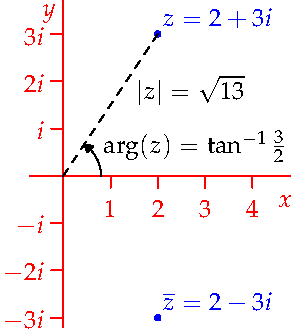
\includegraphics[scale=0.9]{complex-argand}
\end{defn}

\footnotetext{In the language of linear algebra, $\C$ is a vector space over $\R$ with basis $\{1,i\}$.}

\emph{Addition}, \emph{scalar multiplication} (by real numbers) and \emph{complex multiplication} follow the usual algebraic rules while using $i^2=-1$ to simplify.

\begin{example}{}{}
	A simple example of multiplication of complex numbers:
	\begin{align*}
		(2+3i)(4+5i)&=2\cdot 4+2\cdot 5i+3i\cdot 4+3i\cdot 5i\tag{multiply out}\\
		&=8+10i+12i-15 \tag{use $i^2=-1$ to simplify}\\
		&=-7+22i
	\end{align*}
\end{example}

The algebra screams \emph{geometry}! Definition \ref{defn:complexnumbers} already length, angle and reflection in the real axis. Two other aspects of basic geometry are immediate:
\begin{itemize}%\itemsep0pt
  \item Addition by $z$ \emph{translates} all points by $z$.
  \item Scalar multiplication \emph{scales} distances from the origin (similarity).
\end{itemize}
The algebraic property distinguishing the complex numbers from the standard Cartesian plane is \emph{complex multiplication.} To start visualizing this, consider multiplication by $i$,
\[
	iz=i(x+iy)=-y+ix
\]
This is the result of \emph{rotating} $z$ counter-clockwise $\frac\pi 2$ radians about the origin. To obtain all rotations and reflections, we need an alternative description of a complex number.

\begin{lemm}{}{euler}
	\exstart (Euler's Formula)\lstsp For any $\theta\in\R$, $e^{i\theta}=\cos\theta+i\sin\theta$. 
	\begin{enumerate}\setcounter{enumi}{1}
	  \item (Exponential laws)\lstsp$e^{i\theta}e^{i\phi}=e^{i(\theta+\phi)}$ and $(e^{i\theta})^n=e^{in\theta}$ for any $n\in\Z$.
	\end{enumerate}
\end{lemm}

Evaluating at $\theta=\pi$ yields the famous \emph{Euler identity} $e^{i\pi}=-1$. Part 1 can be taken as a definition. To see that it is a reasonable definition requires either power series or elementary differential equations, topics best described elsewhere. Part 2 is an exercise.

\goodbreak


\begin{defn}[lower separated=false, sidebyside, sidebyside align=top seam, sidebyside gap=0pt, righthand width=0.34\linewidth]{}{}
	Let $z=x+iy$ be a non-zero complex number.\smallbreak
	Writing $x=r\cos\theta$ and $y=r\sin\theta$, we obtain the \emph{polar form}
	\[
		z=re^{i\theta}=r(\cos\theta+i\sin\theta)
	\]
	where $r=\nm z$ is the modulus and $\theta=\arg(z)$ the argument of $z$.
	\tcblower
	\flushright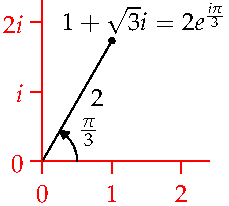
\includegraphics{complex-polar}
\end{defn}

Now consider the effect of multiplying a complex number $z=re^{i\phi}$ by $e^{i\theta}=\cos\theta+i\sin\theta$: according to the Lemma
\[
	e^{i\theta}z=re^{i\theta}e^{i\phi}=re^{i(\theta+\phi)}
\]
which has the same modulus ($r$) as $z$ but a new argument.

\begin{thm}{}{}
	The complex number $e^{i\theta}z$ is the result of rotating $z$ counter-clockwise about the origin through an angle $\theta$.
\end{thm}

\begin{example}{}{}
	To rotate $z=1+2i$ counter-clockwise by $\frac{3\pi}4$ radians, we multiply by\par
	\begin{minipage}[t]{0.69\linewidth}\vspace{-5pt}
	\[
		e^{\frac{3\pi i}4}=\cos\frac{3\pi}4+i\sin\frac{3\pi}4=\frac 1{\sqrt 2}(-1+i)
	\]
	to obtain
	\[
		e^{\frac{3\pi i}4}z =\frac 1{\sqrt 2}(-1+i)(1+2i)=-\frac 1{\sqrt 2}(3+i)
	\]
	\end{minipage}
	\hfill
	\begin{minipage}[t]{0.3\linewidth}\vspace{-15pt}
		\flushright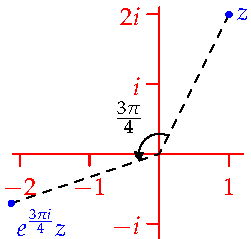
\includegraphics{complex-rotate}
	\end{minipage}\medbreak
	You could try to keep things in polar form, though it doesn't result in a nice answer:
	\[
		z=\sqrt 5e^{i\tan^{-1}2}\implies e^{\frac{3\pi i}4}z=\sqrt 5e^{\frac{3\pi i}4+i\tan^{-1}2}
	\]
\end{example}




\begin{minipage}[t]{0.73\linewidth}\vspace{0pt}
	Reflections may be described by combining rotations with complex conjugation. To reflect across the line making angle $\theta$ with the positive real axis, we rotate the plane so that the reflection appears to be vertical:
	\begin{enumerate}\itemsep0pt
	  \item \textcolor{Green}{Rotate} the plane \emph{clockwise} by $\theta$, that is $z\mapsto e^{-i\theta}z$.
	  \item \textcolor{orange}{Reflect} across the real axis by complex conjugation.
	  \item \textcolor{blue}{Rotate} counter-clockwise by $\theta$.
	\end{enumerate}
	Combining these steps gives the formula.
\end{minipage}
\hfill
\begin{minipage}[t]{0.26\linewidth}\vspace{-5pt}
		\flushright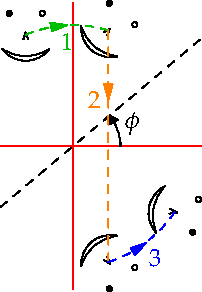
\includegraphics{complex-reflect}
\end{minipage}

\begin{thm}{}{}
	To reflect $z$ across the line making angle $\theta$ with the positive real axis, we compute
	\[
		z\mapsto e^{i\theta}(\cl{e^{-i\theta}z})=e^{2i\theta}\cl z
	\]
\end{thm}

\goodbreak

\begin{example}{}{}
	Reflect $z=-2+3i$ across the line through the origin and $w=\sqrt 3+i$.\smallbreak
	First compute $\theta=\arg(w)=\tan^{-1}\frac 1{\sqrt 3}=\frac\pi 6$. The desired point is therefore
	\[
		e^{\frac{i\pi}3}(-2-3i)=\left(\frac 12+\frac{\sqrt 3}2i\right)(-2-3i) =\left(\frac{3\sqrt 3}2-1\right)-\left(\sqrt 3+\frac 32\right)i
	\]
\end{example}

To describe general rotations and reflections about arbitrary points/lines, we combine our approach with \emph{translations} (compare Exercise \ref*{sec:klein}.\ref{exs:genrotref}).


\begin{cor}{}{fullrotref}
	\exstart To rotate $z$ by $\theta$ about a point $w$, compute $z\mapsto e^{i\theta}(z-w)+w$.
	\begin{enumerate}\setcounter{enumi}{1}
	  \item To reflect $z$ across the line with slope $\theta$ through a point $w$, compute $z\mapsto e^{2i\theta}(\cl z-\cl w)+w$.
	\end{enumerate}
\end{cor}

\begin{example}{}{complexcombi}
	The combination of translation by $-i$, rotation by $\frac\pi 3$ around the origin, then translation by 1, may be expressed
	\[
		z\mapsto e^{\frac\pi 3}\bigl(z-i\bigr)+1=\textcolor{blue}{i+e^{\frac\pi 3}\bigl(z-i\bigr)}+\textcolor{red}{1-i}
	\]
	Alternatively, this is \textcolor{blue}{rotation} by $\frac\pi 3$ around $i$ followed by \textcolor{red}{translation} by $1-i$.
\end{example}

\bigskip


We have now described all the Euclidean isometries of the previous section in the language of complex numbers. Here is the full dictionary.\footnote{Scaling isn't an isometry, but it is worth including nonetheless!}
\begin{center}
	\begin{tabular}{c|c|c}
		Isometry/Transformation
		&
		Complex numbers
		&
		Matrices/vectors
		\\\hline
		Addition/Translation
		&
		$z+w=(x+iy)+(u+iv)$
		&
		$\vz+\vw=\twovec xy+\twovec uv$
		\\
		Scaling
		&
		$\lambda z=(\lambda x)+i(\lambda y)$
		&
		$\lambda\vz=\twovec{\lambda x}{\lambda y}$
		\\
		Rotation CCW by $\frac\pi 2$
		&
		$z\mapsto iz$
		&
		$\vz\mapsto
		\begin{pmatrix}
			0&-1\\
			1&0
		\end{pmatrix}
		\vz$
		\\
		Rotation CCW by $\theta$
		&
		$z\mapsto e^{i\theta}z$
		&
		$\vz\mapsto
		\begin{pmatrix}
			\cos\theta&-\sin\theta\\
			\sin\theta&\cos\theta
		\end{pmatrix}
		\vz$
		\\
		Vertical reflection
		&
		$z\mapsto \cl z$
		&
		$\vz\mapsto
		\begin{pmatrix}
			1&0\\
			0&-1
		\end{pmatrix}
		\vz$
		\\
		Reflection across line with slope $\frac\theta 2$
		&
		$z\mapsto e^{i\theta}\cl z$
		&
		$\vz\mapsto
		\begin{pmatrix}
			\cos\theta&\sin\theta\\
			\sin\theta&-\cos\theta
		\end{pmatrix}
		\vz$
	\end{tabular}
\end{center}

It is perhaps surprising to modern readers, but complex numbers came before vectors and matrix-geometry! During the 1800s mathematicians tried unsuccessfully to replicate the complex number approach in higher dimensions. This ultimately led (via Hamilton's quaternions) to the adoption of vectors and linear algebra/matrix calculations.\smallbreak

One reason for the desire to keep the complex number description is that it may be used to describe further (non-isometric) transformations of the plane: for instance $z\mapsto\cl z^{-1}$ is \emph{reflection in a circle}! We'll discuss some of this at the end of Chapter \ref{chap:hyper}.

\begin{exercises}
	\exstart Use complex numbers to compute the result of the following transformations: you can answer in either standard or polar form.
	\begin{enumerate}\setcounter{enumi}{1}
	% 	\item[]\begin{enumerate}
				%\item Express each of the following fractions as complex numbers by rationalizing the denominator (multiplying through by the complex conjugate\ldots)
	    	%\[\frac 1{2i},\qquad \frac{1+i}{1-i},\qquad \frac 1{2+4i}\]
	%     \item Prove that $\C$ is closed under multiplicative inverses: i.e., $\forall z\in\C\setminus\{0\}$, prove that $\frac 1z\in\C$.
	%   \end{enumerate}
	  \item[]\begin{enumerate}
	    \item Rotate $3-5i$ counter-clockwise around the origin by $\frac{3\pi}4$ radians.
	    \item Reflect $2-i$ across the line joining $1+i\sqrt 3$ and the origin.
	    \item Reflect $1+i$ across the line through the origin making angle $\frac\pi 5$ radians with the positive real axis.
	  \end{enumerate}
	  
	  
	  
	  \item Find the reflection of the point $(2,3)$ across the line making angle $\frac{3\pi}8$ with the positive $x$-axis. Give your answer using both complex numbers and matrices/vectors.
	  
	  
		\item Repeat the previous question for the point $(3,4)$ and the angle $\frac{5\pi}{12}=\ang{75}$.
	  
	  
	  \item Describe the geometric effect of the map $z\mapsto \frac 1{\sqrt 2}(-1-i)\bigl(\cl z-3+4i\bigr)$.\par
	  (\emph{Hint: compare Example \ref{ex:complexcombi}})
	  
	  
	  \item (Hard)\lstsp Consider the line $\ell$ through the origin and $\bigl(\sqrt{2+\sqrt 2},\sqrt{2-\sqrt 2}\bigr)$. Compute the result of reflecting $-2+3i$ across $\ell$.
	    
	      
	  \item By letting $n=3$ in Lemma \ref{lemm:euler}, prove that 
	  	\[\cos 3\theta=4\cos^3\!\theta-3\cos\theta\]
	  	Find a corresponding trigonometric identity for $\sin 3\theta$.
	  	
	  	
	  \item Prove part 2 of Lemma \ref{lemm:euler}.\par
	  (\emph{Hint: use the multiple-angle formulae (page \pageref{sec:multangle}) to expand $e^{i(\theta+\phi)}$})
	  	
	 	%\item Prove Corollary \ref{cor:fullrotref}.%\par
	 	%(\emph{Hint: translate $w$ to the origin, rotate/reflect, then translate back})
	 	
	\end{enumerate}
 	
  
  
  
%   \item[] \emph{The last questions are on the stereographic projection. Remember that this is completely optional!}
%   
%   \item\begin{enumerate}
%     \item Prove that $x,y\in\Q\iff X,Y,Z\in\Q$ so that rational points on the sphere $S^2\setminus\{N\}$ correspond to rational points in $\C$.
%     \item Find some examples of `Pythagorean' quadruples: $a,b,c,d\in\N$ such that $a^2+b^2+c^2=d^2$.\\
%     (\emph{Hint: if $(X,Y,Z)$ is a rational point on the sphere\ldots You might want to start by finding some standard Pythagorean triples which correspond to $Y=0$.})
%   \end{enumerate}
%   
%   \item A circle in the sphere is defined as the intersection of a plane $aX+bY+cZ=d$ with the sphere $X^2+Y^2+Z^2=1$.
%   \begin{enumerate}
%     \item Prove that the plane intersects the sphere in a circle if and only $d^2<a^2+b^2+c^2$.
%     \item Check that the circle passes through the north pole if and only if $c=d$. In this case prove that the stereographic projection of the circle in $S^2$ is a line in $\C$.\footnote{The corresponding line in the plane may be thought of as a circle passing through $\infty$.} Argue that \emph{every} line in $\C$ corresponds to a circle in $S^2$.
%     \item If $c\neq d$ prove that
%     \[\left(x-\frac a{d-c}\right)^2+\left(y-\frac b{d-c}\right)^2=\frac 1{(d-c)^2}(a^2+b^2+c^2-d^2)\]
%     so that the stereographic projection is a circle in $\C$. Again, argue that the converse is true: every circle in $\C$ inverse projects to a circle in $S^2$ which does not pass through the north pole.
%   \end{enumerate}
%    
%   \item\begin{enumerate}
%     \item Consider the circle $(x-5)^2+(y-3)^2=1$ in $\C$. Prove that the inverse projection of this circle onto $S^2$ lies on the plane
%     \[5X+3Y+16Z=17\tag*{($\ast$)}\]
%     \item Find the inverse projection of the center $(5,3)$ of the circle in part (a).
%     \item The center of the circle on $S^2$ from part (a) is the point whose position vector is the unit normal vector of the plane ($\ast$): \emph{think about the picture!}. Compare this to your answer to part (b). What do you observe?
%     \item Suppose that a circle $C_1$ in $\C$ corresponds under the stereographic projection to a circle $C_2$ in the sphere. Prove the following:\\
%     The centers of $C_1$ and $C_2$ correspond under stereographic projection if and only if $C_1$ is centered at the origin and has radius $r\le 1$. 
% 	\end{enumerate}
% 	
% 	\item (Needs some multi-variable calculus!) Consider the inverse projection $\vr:\C\to S^2$ used as a parametrization of the sphere $S^2$:
% 	\[\vr(x,y)=\frac{1}{x^2+y^2+1}\sthreevec{2x}{2y}{x^2+y^2-1}\]
% 	\begin{enumerate}
% 	  \item Compute the tangent vectors $\vr_x$ and $\vr_y$ for this parametrization and prove that
% 	  \[\vr_x\cdot\vr_x=\vr_y\cdot\vr_y=\frac 4{(x^2+y^2+1)^2}\qquad \vr_x\cdot\vr_y=0\]
% 	  This says that $x,y$ are \emph{orthogonal co-ordinates} for the sphere, but that they do not preserve length ($\nm{\vr_x}$ varies depending on the location $(x,y)$).
% 	  \item Consider two small changes in $(x,y)$: $(x,y)+(\dx_1,\dy_1)$ and $(x,y)+(\dx_2,\dy_2)$. The resulting tangent vectors to the surface of $S^2$ are then
% 		\[\D\vu=\vr_x\,\dx_1+\vr_y\,\dy_1,\qquad\D\vv=\vr_x\,\dx_2+\vr_y\,\dy_2\]
% 		Use the formula $\cos\theta=\frac{\D\vu\cdot\D\vv}{\nm{\D\vu}\nm{\D\vv}}$ to compare the \emph{angle} between these tangent vectors to the angle between the vectors $\stwovec{\dx_1}{\dy_1}$ and $\stwovec{\dx_2}{\dy_2}$. What do you observe?
% 		\item Compute the \emph{area element} $\dS=\nm{\vr_x\times\vr_y}\dx\,\dy$ for this parametrization. You should conclude that the projection distorts areas relative to those in $\C$: a small area near the top of the sphere corresponds to a large area far away from the origin in $\C$.
% 	\end{enumerate}
\end{exercises}

\clearpage


\subsection{Birkhoff's Axiomatic System for Analytic Geometry (non-examinable)}

Recall that analytic geometry, as developed by Descartes and Fermat, was originally conceived as a bolt-on to Euclidean geometry. In 1932 George David Birkhoff %\footnote{%
%	The instructor's great-great-grand-advisor!
%} 
provided an axiomatization of analytic geometry in its own right. %


\boldinline{Background}

Assume the usual properties/axioms of the real numbers as a complete ordered field. Birkhoff's approach is typical of modern axiomatic systems in that it is built on top of pre-existing systems (set theory, complete ordered fields, etc.).

\boldinline{Undefined terms}

Two objects: \emph{Point, line.} Two functions: \emph{distance $d$, angle measure $\measuredangle$.} If the set of points is $\cS$, then,
\[
	d:\cS\times\cS\to\R^+_0,\qquad \measuredangle:\cS\times\cS\times\cS\to [0,2\pi)
\]


\boldinline{Axioms}

\emph{Euclidean}\lstsp Given two distinct points, there exists a unique line containing them.
\begin{description}%\itemsep0pt
  \item[\normalfont\emph{Ruler}] Points on a line $\ell$ are in bijective correspondence with the real numbers in such a way that if $t_A,t_B$ correspond to $A,B\in\ell$, then $\nm{t_A-t_B}=d(A,B)$.
  \item[\normalfont\emph{Protractor}] The rays emanating from a point $O$ are in bijective correspondence with the set $[0,2\pi)$ so that if $\alpha$, $\beta$ correspond to rays $\ray{OA}$, $\ray{OB}$, then $\measuredangle AOB\equiv \beta-\alpha\pmod{2\pi}$. This correspondence is continuous in $A,B$.
  \item[\normalfont\emph{SAS similarity}]\!\!\footnote{%
		As with Hilbert, Birkhoff makes SAS an \emph{axiom}: Birkhoff's version is stronger in that it also applies to similar triangles.%
	}\, If $\triangle ABC$ and $\triangle XYZ$ satisfy $\measuredangle ABC=\measuredangle XYZ$ and $\frac{d(A,B)}{d(X,Y)}=\frac{d(B,C)}{d(Y,Z)}$, then the remaining angles have equal measure and the final sides are in the same ratio (i.e., $\triangle ABC\sim\triangle XYZ$).
\end{description}

\boldinline{Definitions} As with Hilbert, some of these are required before later axioms make sense. In particular, the definition of \emph{ray} is required before the \emph{protractor} axiom.
\begin{description}
	\item[\normalfont\emph{Betweenness}] $B$ lies between $A$ and $C$ if $d(A,B)+d(B,C)=d(A,C)$
  \item[\normalfont\emph{Segment}] $\overline{AB}$ consists of the points $A,B$ and all those between
  \item[\normalfont\emph{Ray}] $\ray{AB}$ consists of the segment $\cl{AB}$ and all points $C$ such that $B$ lies between $A$ and $C$.
  \item[\normalfont\emph{Basic shapes}] Triangles, circles, etc.
\end{description}



\boldsubsubsection{Analytic Geometry as a Model}

The axioms should feel familiar. Being shorter than Hilbert's list, and being built on familiar notions such as the real line, it is somewhat easier for us to understand what the axioms are saying and to visualize them. There is something to \emph{prove} however; indeed the major point of Birkhoff's system!

\begin{thm}{}{}
	Cartesian analytic geometry is a model of Birkhoff's axioms.
\end{thm}

Recall what this requires: we must provide a \emph{definition} of each of the undefined terms and prove that these satisfy each of Birkhoff's axioms. Here are suitable definitions for Cartesian analytic geometry:
\begin{description}
	\item[\normalfont\emph{Point}] An ordered pair $(x,y)$ of real numbers.
	\item[\normalfont\emph{Distance}] $d(A,B)=\sqrt{(A_x-B_x)^2+(A_y-B_y)^2}$
	\item[\normalfont\emph{Line}] All points satisfying a linear equation $ax+by+c=0$.
	\item[\normalfont\emph{Angle}] Define column vectors as differences ($\vv=P-O$ and $\vw=Q-O$) and consider the matrix $J=
	\begin{smatrix}
		0&-1\\
		1&0
	\end{smatrix}$. 
	Now define angle via
	\[
		\cos\measuredangle POQ=\frac{\vv\cdot\vw}{\nm{\vv}\nm{\vw}}
		\quad\text{where}\quad
		\measuredangle POQ\in
		\begin{cases}
			[0,\pi]&\iff\vw\cdot J\vv\ge 0\\
			(\pi,2\pi)&\iff\vw\cdot J\vv< 0
		\end{cases}
		\tag{$\ast$}
	\]
	In essence $J$ is `rotate counter-clockwise by $\frac\pi 2$.' Cosine may be defined using power series, so no pre-existing geometric meaning is necessary.
\end{description}

\begin{proof}
	(Euclidean axiom)\quad If $(x_1,y_1)$ and $(x_2,y_2)$ satisfy $ax+by+c=0$ then
	\[
		a(x_1-x_2)+b(y_1-y_2)=0
	\]
	whence $a=y_1-y_2$, $b=x_2-x_1$ up to scaling. It follows that the line has equation
	\[
		(y_1-y_2)x+(x_2-x_1)y+x_1y_2-x_2y_1=0
	\]
	unique up to multiplication of all three of $a,b,c$ by a non-zero constant.\smallbreak
	The remaining axioms are exercises.
\end{proof}


\begin{exercises}
	\exstart Prove that the ruler axiom is satisfied:
	\begin{enumerate}\setcounter{enumi}{1}
	  \item[]\begin{enumerate}
	    \item First show that if $P\neq Q$ lie on $\ell$, then any point $A$ on the line has the form
			\[
				A=P+\frac{t_A}{d(P,Q)}(Q-P)
				\qquad\text{where }
				t_A\in\R
			\]
			\item Use this formula to verify that $d(A,B)^2=(t_A-t_B)^2$.
		\end{enumerate}
		
		\item Let $\vi=\stwovec 10$. Given any non-zero point $B$, define $\vb=B-O$ and let $\beta=\cos^{-1}\frac{\vi\cdot\vb}{\nm{\vb}}$ in accordance with $(\ast)$. This is a continuous function of $\vb$.
		\begin{enumerate}
		  \item If $\hat B$ is any other point on the same ray $\ray{OB}$, explain why we get the same value $\beta$.\par
		  (\emph{$\beta$ is thus a continuous function of $B$})
		  \item If $B=(x,y)$, what are values $\cos\beta$ and $\sin\beta$?
		  \item	Suppose $A$ corresponds to $\alpha$ under this identification. Evaluate $\cos(\beta-\alpha)$ and therefore prove that the protractor axiom is satisfied.
		\end{enumerate}
		
		\item Use the cosine rule (Theorem \ref{thm:cosinerule}) to prove that the SAS similarity axiom is satisfied.
	\end{enumerate}
\end{exercises}

